
\chapter{First-Class Labels}
\label{ch:first-class-labels}

The interpreter portion of \JitFlow\ forms the foundation of an information-flow tracking web browser that tracks flow in the Document Object Model, named ConDOM~\cite{kerschbaumer.etal+12}.
A modification of the ConDOM browser that randomly switches the information flow tracking capabilities on and off later formed a critical component of a system, called CrowdFlow~\cite{kerschbaumer.etal+13}, that gathers attack statistics across a crowd of users.

Concordant with our attack model (\autoref{ch:defense}), these systems also define an \emph{information leak} as the communication of any information to a web origin that differs from the flow-tracked derivation of that information.
Through automated browsing, ConDOM and CrowdFlow discovered a high number of false positives, where the web application sourced much of its material from Content Distribution Networks (CDNs) that have different domains than the page itself.

These observations indicate that JavaScript program authors have more knowledge about the information-flow security needs of the application they develop than any automated system can assess~\cite{hennigan.etal+12, hennigan.etal+13}.
To combat label creep and preempt the ex-post suggestion of applying a policy that whitelists CDNs, \JitFlow\ exposes some of the internal labeling operations through a first-class language feature.
Using this API, the JavaScript programmer, armed with domain knowledge, gains the ability to tag specific, security sensitive, values within their application.
By reducing the number of sources for labels, the developer can delay and mitigate the encroachment caused by label creep.

In addition to the tracking capabilities already outlined, \JitFlow\ also presents reflective \FlowLabel\ objects to interface with an internal \FlowLabelRegistry\ that holds the label lattice (\autoref{sec:label-lattice}).
The \FlowLabel\ objects themselves come equipped with \mjoin\ and \msubsumes\ methods that facilitate the composition and comparison of labels.
A keyword operator, \mlabelof, enables accessing the label attached to a program value.
Together these features enable developers to express security policies written in their native tongue, JavaScript.

\section{Benefits of First-Class Labeling}

%The web application developer can use the first-class labeling to label only those values which the application considers sensitive.
%This selective labeling programmatically focuses the reporting of unauthorized information flows within a web application, reducing the number of false positives that have prevented adoption of other information flow systems~\cite{sabelfeld.myers+03}.

Other systems implementing information flow within a web browser~\cite{jang.etal+10,meyerovich.livshits+10,just.etal+11} attempt to create a fully automatic labeling system, with no feedback from the application developer.
Researchers intend for the automatic application of labels to provide easy migration of existing code bases, but, in reality, the approach increases the number of false positives and policy violation warnings~\cite{sabelfeld.myers+03, slowinska.bos+09}
Because privacy concerns remain application specific, we find the automatic approach naively optimistic.

Without some domain knowledge assistance, automated labeling frameworks detect and report information flows, such as requests from content distribution servers, that application developers would like to disregard.
By selectively tagging only those variables considered security sensitive, developers can focus their attention on flows of specific information, and avoid sifting through the morass of false positive reports generated by automated labeling systems.
We do not think that information flow techniques will see adoption without the ability to selectively ignore these flow reports in a flexible developer-controlled manner.
With the first-class labeling features, \JitFlow\ provides developers a custom JavaScript engine that can answer questions about information flows in their application, such as ``Does the user-entered password field influence network requests to third parties, potentially leaking information?'' and ``What other objects might this field influence?''

The implementation of first-class labels does not incur any significant execution performance penalty (\autoref{sec:first-class-performance}).
The design resists JavaScript-level attacks against itself, even while exposing the underlying security data structures.
While we do not expect all clients to update their browsers to include the \JitFlow\ information flow tracking engine, developers can still benefit by using the first-class label feature as a debug environment to detect existing web application security holes.

\section{Supporting Framework}
\label{sec:supporting-framework}

The dynamic information-flow labeling internals implemented in \JitFlow\ (\autoref{ch:label-propagation}) provides the foundation for the first-class labeling system presented in this chapter.
The labeling framework supports the runtime creation and application of labels because security principals represented on a web page, because these principals do not become known to the browser and \JitFlow\ until a user visits the page.
Every JavaScript value carries a label representing an element from the finite powerset lattice over principals.
\JitFlow\ conservatively labels the result of every operation with the union (join) of the labels of its inputs, monotonically moving up the lattice of security principals.
To prevent attack code from removing or downgrading the labels applied to values tracked by the VM, the labeling framework does not currently provide a mechanism for declassification (i.e., it does not expose an intersection (meet) operation).

\begin{figure*}[t]
 \centering
 \resizebox{\textwidth}{!}{
\begin{tikzpicture}[
    node distance = 1cm, auto,
    force/.style={rectangle, inner sep=5pt, text badly centered, minimum height=.8cm},
    every text node part/.style={align=center},
    ]

    \begin{scope}[yshift=4.0cm, xshift=-7.5cm]
    \node[shape=rectangle, draw] {
       \begin{tabular}{l|c}
          \multicolumn{2}{c}{\FlowLabelRegistry\ mapping} \\
          \hline
          \codestringdbl{example.com} & \texttt{0001} \\
          \codestringdbl{pwd} & \texttt{0010} \\
          \codestringdbl{ad.com} & \texttt{0100} \\
       \end{tabular}
    };
    \end{scope}

    \begin{scope}
    \matrix[nodes={force}, column sep=1cm, ampersand replacement=\&] {
        \node (ex) {\codestringdbl{example.com}\\ \code{0001}}; \&
        \node (mp) {\codestringdbl{pwd}\\ \code{0010}}; \&
        \node (ad) {\codestringdbl{ad.com}\\ \code{0100}}; \\
    };
    \end{scope}

    \begin{scope}[yshift=2cm]
    \matrix[nodes={force}, column sep=.5cm, ampersand replacement=\&] {
      \node (exUmp) {\codestringdbl{example.com} $\sqcup$ \codestringdbl{pwd}\\ \code{0011}}; \&
      \node (exUad) {\codestringdbl{example.com} $\sqcup$ \codestringdbl{ad.com}\\ \code{0101}}; \&
      \node (mpUad) {\codestringdbl{pwd} $\sqcup$ \codestringdbl{ad.com}\\ \code{0110}}; \\
    };
    \end{scope}

    \begin{scope}[yshift=4cm]
    \matrix[nodes={force}, column sep=1cm] {
      \node (exUmpUad) {\codestringdbl{example.com} $\sqcup$ \codestringdbl{pwd} $\sqcup$ \codestringdbl{ad.com}\\ \code{0111}}; \\
    };
    \end{scope}

%    \begin{scope}[yshift=-1.5cm]
%    \matrix[nodes={force}, column sep=1cm] {
%      \node (base) {$\perp$\\ \code{0000}};\\
%    };
%    \end{scope}

    \draw[arrow] (ex) -- (exUmp);
    \draw[arrow] (ex) -- (exUad);

    \draw[arrow] (mp) -- (exUmp);
    \draw[arrow] (mp) -- (mpUad);

    \draw[arrow] (ad) -- (exUad);
    \draw[arrow] (ad) -- (mpUad);

    \draw[arrow] (exUmp) -- (exUmpUad);
    \draw[arrow] (exUad) -- (exUmpUad);
    \draw[arrow] (mpUad) -- (exUmpUad);

%    \draw[arrow] (base) -- (ex);
%    \draw[arrow] (base) -- (mp);
%    \draw[arrow] (base) -- (ad);

\end{tikzpicture}
}
 \caption{The \FlowLabelRegistry\ mapping three JavaScript strings used as security principals to unique bit positions.
   These principals form a lattice of security labels, represented as bit vectors.}
 \label{fig:flowlabel-lattice}
\end{figure*}

\subsection{Storage of Security Principals and Labels}
\label{sec:label-storage}

The underlying labeling framework allows any JavaScript value to be used as a security principal, although all examples will use strings.
The first-class labeling system merely exposes this ability as a concise labeling API to the JavaScript developer.
As we shall see (\autoref{sec:using-first-class-labels}), the ability to use any JavaScript value as a principal gives web authors enough power to represent security principals as a native part of an application's code.

The supporting information flow VM interns every JavaScript value used as a security principal in the \FlowLabelRegistry, mapping it to a unique bit position.
\autoref{fig:flowlabel-lattice} depicts the interning of three JavaScript string objects, \codestringdbl{example.com}, \codestringdbl{pwd}, and \codestringdbl{ad.com}, each representing a security principal in the \FlowLabelRegistry.
To minimize the attack surface on the system itself, the first-class extensions (\autoref{sec:first-class-implementation}) do not make this data structure accessible to the JavaScript programmer.

As shown in \autoref{fig:flowlabel-lattice}, the mapping held by the \FlowLabelRegistry\ allows a bit vector to represent each security label.
\JitFlow\ attaches a security label to every JavaScript value, representing an element from a powerset lattice over security principals.
The current implementation of the underlying information flow framework does not support more than 64 unique principals, due to the bit vector representation of labels (\autoref{sec:existing-type-system} and \autoref{sec:label-storage}).
However, experiments surfing the web have not found this limitation to be a problem in practice (\autoref{sec:first-class-evaluation}).

\subsection{Attack Surface and Example Attack Code}
\label{subsec:attack}

The modifications that \JitFlow\ makes to perform information flow tracking at the VM level allows the first-class labeling feature to avoid potential attacks on the tracking system itself.
This design reduces the size of the attack surface compared to JavaScript rewriting systems~\cite{chugh.etal+09, jang.etal+10}.

Exposing \JitFlow's underlying framework through the first-class labeling API might create a new attack surface (targeting the underlying label framework itself) meant to be hidden by design.
As a result of this concern, the first-class labeling system does not support declassification.
Both the JavaScript developer and any potential JavaScript attack code can only create, apply, and inspect labels, but cannot remove them.
During computation, these labels may walk their way monotonically up the label lattice.

\lstset{
  caption={Password sniffing via active implicit information flow.},
  label={list:sniffPassword}
}
\begin{jscode}
function sniffPassword(pw) {
  var spw = "";
  for (var i = 0; i < pw.length; i++) {
    switch(pw[i]) {
    case 'a': spw += 'a'; break;
    case 'b': spw += 'b'; break;
    ... // other characters elided
    }
  }
  return spw;
}
\end{jscode}

\autoref{list:sniffPassword} gives an example of an attacker provided function which attempts to drop any label attached to the argument~\code{pw}.
\JitFlow's label framework can track the control-flow dependence of the return variable (\code{spw}) on the argument (\code{pw}) at both the loop condition (\code{pw.length}) and the switch condition (\code{pw[i]}).
By performing such tracking, the returning variable~\code{spw} subsumes the same set of principals as the incoming function argument~\code{pw}.
The tracking and propagation rules enforced by \JitFlow\ prevent the attacker from dropping labels through active implicit information leaks in exfiltration code.

\subsection{Information Flow in the Browser}

To execute the motivating example and demonstrate the power of information flow tracking, the first-class labeling resides in a modified web browser environment that hosts the tracking VM \JitFlow\ together with additional subsystems for information storage, rendering, document description, and network communication.
These other subsystems represent covert channels through which an attacker may communicate information.
To provide a starting basis, the web browser automatically applies labels to dynamically loaded code and resources according to the site of origin.

In addition to storing visible page elements, the Document Object Model (DOM) allows creation of invisible elements within the document that can be used to store and communicate information.
The modified web browser propagates labels to HTML elements and attributes within the DOM so that an attacker cannot use it as a channel to remove labels.

The information flow tracking web browser also contains a network monitor that observes the labels on all network traffic: dynamic requests for remote resources such as images and stylesheets, HTTP GET and POST methods for forms, and \code{XmlHttpRequest} for AJAX.
\JitFlow's first-class labeling system presents to the web developer a mechanism for registering JavaScript functions which implements network monitor logic, enabling the developer write code that inspects labels attached to resource requests, thereby discovering information leaks.

\section{Design and Implementation of First-Class Labels}
\label{sec:first-class-implementation}

Before discussing the first-class label interface that a JavaScript developer uses to hook into the supporting information flow framework, we first give details explaining the extensions and modifications necessary to support labels as first-class JavaScript objects.

\subsection{Reflecting Labels into JavaScript}
The supporting framework contains a \FlowLabelRegistry\ that maps primitive values and JavaScript objects used as principals to a position within a bit vector label.
By holding a reference to every JavaScript object (within the standard heap) used as a principal, the \FlowLabelRegistry\ keeps it alive during garbage collection.
Assignment of principals to bit vector positions prevents the \FlowLabelRegistry\ from releasing principals for re-use.
Doing so would introduce ambiguity in the mapping from labels to web domains.

The first-class labeling feature reflects the underlying labels into the JavaScript language, as native JavaScript objects, via the \FlowLabelObject\ wrapper.
When reflected into JavaScript as \FlowLabelObject\ instances, security labels can themselves be labeled and can also act as security principals, just like any other JavaScript value.
Additionally, they act as callable objects, providing an interface to apply the internally stored label onto any given argument value.
In the interest of clarity, we do not use any examples that exhibit the inherent recursive nature of the first-class labeling system, and restrict the examples to use only strings as security principals.

\begin{figure}[ht]
  \centering
\begin{tikzpicture}
  \node (proto) [rectangle split, rectangle split part align=left, rectangle split parts=2,
      draw, text width=5.2cm] {
      \FlowLabel\ Prototype
  \nodepart{second}
      \texttt{+} \bracketdbl{toString}\\
      \texttt{+} \bracketdbl{construct}\\
      \texttt{+} \mjoin\\
      \texttt{+} \msubsumes
  };

  \node (obj) [below=1cm of proto.south, anchor=north,
      rectangle split, rectangle split part align=left, rectangle split parts=2,
      draw, text width=5.2cm]
  {
      \FlowLabelObject
  \nodepart{second}
      \texttt{+} \bracketdbl{call}
  };

  \draw[-open triangle 45, style=dotted] (obj.north) -- node[near start,right] {\texttt{-}\bracketdbl{prototype}} (proto.south);

\end{tikzpicture}
  \caption{UML class diagram of the first-class labeling system that introduces the \FlowLabel\ prototype constructor, and \FlowLabelObject\ instances.
  As in the ECMA~\cite{ecma} language standard, \bracketdbl{\textbullet} indicates implementation internal methods.}
  \label{fig:uml}
\end{figure}

The first-class labeling system also introduces a singleton \FlowLabel\ prototype that both holds methods common to all \FlowLabelObject\ instances and provides an interface through which the JavaScript developer can construct \FlowLabelObject s.
These first-class objects wrap the security labels propagated by \JitFlow\ and provide the developer an interface for label composition and application.
\autoref{fig:uml} uses UML to depict the relationship between the \FlowLabel\ prototype singleton and \FlowLabelObject\ instances.

\subsection{JavaScript Syntax Extension to Retrieve Labels}

The first-class labeling system implements a small change to the JavaScript language permitting JavaScript code to retrieve a label from a given value.
It introduces the keyword \mlabelof, as a new case in the \UnaryExpression\ grammar rule of the ECMA~\cite{ecma} language standard.
\autoref{fig:labelof} presents the entire grammar rule, including boldface emphasis on the new language keyword.

\begin{figure}[ht]
  \centering
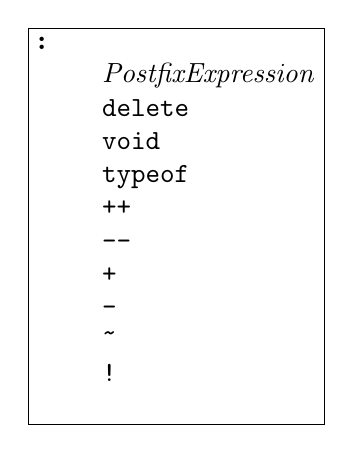
\begin{tikzpicture}
  \node (syntax) [anchor=south east, draw, align=left] {
    \UnaryExpression\textbf{:}\\
    $\hspace{2em}$ \textit{PostfixExpression}\\
    $\hspace{2em}$ \texttt{delete} \UnaryExpression\\
    $\hspace{2em}$ \texttt{void} \UnaryExpression\\
    $\hspace{2em}$ \texttt{typeof} \UnaryExpression\\
    $\hspace{2em}$ \texttt{++} \UnaryExpression\\
    $\hspace{2em}$ \texttt{--} \UnaryExpression\\
    $\hspace{2em}$ \texttt{+} \UnaryExpression\\
    $\hspace{2em}$ \texttt{-} \UnaryExpression\\
    $\hspace{2em}$ \texttt{\textasciitilde} \UnaryExpression\\
    $\hspace{2em}$ \texttt{!} \UnaryExpression\\
    $\hspace{2em}$ \textbf{\mlabelof\ \UnaryExpression}
  };

\end{tikzpicture}
  \caption{Modified JavaScript grammar rule for \UnaryExpression, highlighting the introduction of the \mlabelof\ keyword.}
  \label{fig:labelof}
\end{figure}
\vspace*{-\baselineskip}

\subsection{Network Hook in the Web Browser}

To permit the enforcement of policies written in JavaScript, the browser-hosted JavaScript environment includes one additional change.
Within WebKit, all network traffic conveniently passes through a single network interface class.
A network monitor interface wraps this class and reveals in through a function, \code{registerSendMonitor(fn)}, on the hosted \code{navigator} object.
Using this feature, the web developer can phrase application specific security policies concerning allowed network communication as a JavaScript function within the web application itself.
Once registered, these functions act as network monitors that inspect the payload of all resource requests before being sent over the network.

\section{Using First-Class Labels}
\label{sec:using-first-class-labels}

We design the first-class labeling system and its JavaScript API according to the functional programming paradigm, with the purpose of making it easier for web developers to adopt.
The first-class labeling API contains one minor syntax change to the JavaScript grammar, introducing the new \mlabelof\ operator and keyword.
It also extends the hosted environment (\emph{not} the ECMA specification) with a new built-in \FlowLabel\ prototype constructor object that holds methods for label composition (\mjoin) and comparison (\msubsumes).
Labels take the form of native built-in \FlowLabelObject\ instances, and behave with the same semantics as any other JavaScript object.
\JitFlow's first-class labeling features make a minimal set of changes necessary to expose its internal information flow framework.

The examples in this chapter show how the labeling framework detects and prevents information leakage that might occur due to a script injection attack.
All of the following examples show output of the labeling system at the JavaScript console.
Statements input to the console begin with a `\verb|>|'.
The console describes the resulting value in two parts: the value itself and the label attached to that value.

\subsection{Label Creation}

The first-class labeling extension of \JitFlow\ introduces a \FlowLabel\ prototype singleton to the JavaScript environment hosted by the web browser.
This object implements the internal \bracketdbl{construct} method so that JavaScript code may create first-class label objects.
The web developer may choose any valid JavaScript value to act as a security principal, and pass that value into the constructor.
After interning the provided value in the underlying framework's \FlowLabelRegistry, the constructor returns a \FlowLabelObject\ instance.
In the interest of avoiding attacks on the labeling system itself, \JitFlow's first-class labeling API does not provide programmatic access to the \FlowLabelRegistry.


\lstset{
  caption={Creating a Label Object.},
  label={list:create-label}
}
\begin{jscode}
> pwdLabel = new FlowLabel("pwd");
  [FlowLabelObject pwd] [FlowLabel example.com]
\end{jscode}

\autoref{list:create-label} shows a web developer creating a label using the JavaScript string, \codestringdbl{pwd}, as a security principal.
The web browser hosting \JitFlow\ automatically applies a label to every resource representing its domain of origin.
Consequently, the resulting \FlowLabelObject\ instance returned from the constructor itself carries a label representing the origin of this code snippet: \code{\url{example.com}}.

\subsection{Label Identification}

When the program uses a JavaScript value as a principal in the constructor of a \FlowLabelObject\, \JitFlow\ interns that value in the \FlowLabelRegistry.
Interning the principals allows fast unique identification of labels held by \FlowLabelObject\ instances.

\lstset{
  caption={Label Identity Operator.},
  label={list:identity}
}
\begin{jscode}
> lab1 = new FlowLabel("password");
  [FlowLabelObject password] [FlowLabel example.com]
> lab2 = new FlowLabel("pass" + "word");
  [FlowLabelObject password] [FlowLabel example.com]
> lab1 === lab2
  true [FlowLabel example.com]
\end{jscode}


\autoref{list:identity} shows that \JitFlow\ considers identical two different \FlowLabelObject\ instances constructed with equivalent string values.
As part of the interning process for the second label, \code{lab2}, the \FlowLabelRegistry\ first checks to see if the string argument, \code{"pass" + "word"}, has already been stored.
In this case, the first label, \code{lab1}, has already registered the same value.
The \FlowLabelRegistry\ responds by returning a \FlowLabelObject\ with the same underlying bit vector.
Line~\code{5} performs a comparison of the bit vector label values held by \code{lab1} and \code{lab2}, discovering the strict equality.

\subsection{Label Application}

The \FlowLabelObject\ instance acts as a first-class wrapper object around an internal bit-vector representation of a security label.
The \FlowLabelObject\ instance also implements the internal \bracketdbl{call} method, so that the security label may be attached to other JavaScript values.
When the \FlowLabelObject\ functor receives a passed value, it unions that value's current label with its internally stored label and returns the result.

\lstset{
  caption={Applying a Label to a JavaScript Value.},
  label={list:apply-label},
}
\begin{jscode}
> pass = "24sk09nk12";
  24sk09nk12 [FlowLabel example.com]
> pass = pwdLabel(pass);
  24sk09nk12 [FlowLabel pwd, example.com]
\end{jscode}

\autoref{list:apply-label} shows the JavaScript developer applying the password label constructed previously (\autoref{list:create-label}), \code{pwdLabel}, to a string, \code{pass}.
After label application, the resulting password string carries a label describing both the domain of origin, \code{\url{example.com}}, and the password security principal, \codestringdbl{pwd}.

\subsection{Label Composition}

Behind each \FlowLabelObject\ lies a bit vector representation of a set of principals that describe the label's position in the lattice over principals held by the \FlowLabelRegistry.
The joining of two labels produces a new label that holds the principal set union of its arguments.
\JitFlow\ implements the join operation as an bitwise-or to maintain runtime performance.

\lstset{
  caption={Symmetry of Label Join.},
  label={list:label-join},
}
\begin{jscode}
> lab1 = new FlowLabel("label1")
  [FlowLabelObject label1] [FlowLabel example.com]
> lab2 = new FlowLabel("label2")
  [FlowLabelObject label2] [FlowLabel example.com]
> lab1.join(lab2)
  [FlowLabelObject label1, label2] [FlowLabel example.com]
> lab1.join(lab2) === lab2.join(lab1)
  true [FlowLabel example.com]
\end{jscode}

\autoref{list:label-join} illustrates the programmer composing a new label from two existing labels (Line~\code{5}).
\JitFlow\ makes this functionality readily accessible by supporting an \mjoin\ method on the built-in \FlowLabel\ prototype object.
As shown by the strict equality comparison (Line~\code{7}), the join operation is symmetric.

\subsection{Label Comparison}

In conformance with the lattice definition of subsumption, a label $A$ sumsumes another label $B$, written \code{A.subsumes(B)}, if and only if all of the principals within the second label $B$ also exist within the first label $A$.

\lstset{
  caption={Properties of Label \msubsumes\ Method.},
  label={list:label-subsumes},
}
\begin{jscode}
> lab1 = new FlowLabel("label1")
  [FlowLabelObject label1] [FlowLabel example.com]
> lab2 = new FlowLabel("label2")
  [FlowLabelObject label2] [FlowLabel example.com]
> lab3 = new FlowLabel("label3")
  [FlowLabelObject label3] [FlowLabel example.com]

> lab1.subsumes(lab1)
  true [FlowLabel label1, example.com]

> (lab1.join(lab2)).subsumes(lab2)
  true [FlowLabel example.com]
> (lab1).subsumes(lab1.join(lab2))
  false [FlowLabel example.com]

> (lab1.join(lab2)).subsumes(lab1.join(lab3))
  false [FlowLabel example.com]
\end{jscode}

As shown in \autoref{list:label-subsumes}, all labels subsume themselves (Line~\code{8}).
Labels higher up the lattice only subsume lower ones when it contains all of the lower label's principals (Line~\code{11}), while lower labels can never meet this condition with respect to higher labels (Line~\code{13}).
Finally, labels on the same level of the lattice do not subsume one another (Line~\code{16}).

\subsection{Label Retrieval}

Not only can JavaScript programmers create label objects and apply them to program values, but they can also retrieve a first-class \FlowLabelObject\ from any tagged value.
\JitFlow\ provides the \mlabelof\ operator to accomplish this task.

\lstset{
  caption={Retrieving a Label from a Tagged Value.},
  label={list:label-labelof},
}
\begin{jscode}
> labA = new FlowLabel("labelA")
  [FlowLabelObject labelA] [FlowLabel example.com]
> x = labA("hello")
  hello [FlowLabel labelA, example.com]

> labB = new FlowLabel("labelB")
  [FlowLabelObject labelB] [FlowLabel example.com]
> x = labB(x)
  hello [FlowLabel labelA, labelB, example.com]

> labelof x
  [FlowLabelObject lableA, labelB, example.com]
    [FlowLabel labeA, labeB, example.com]

> (labelof x)("world")
  world [FlowLabel labelA, labelB, example.com]

> (labelof x) === labA.join(labB)
  true [FlowLabel labelA, labelB, example.com]
\end{jscode}

\autoref{list:label-labelof} shows an example usage of the \mlabelof\ operator to retrieve a first-class \FlowLabelObject\ from a program value (Line~\code{11}).
The programmer can then use the resulting \FlowLabelObject\ to apply a label to other values (Line~\code{15)} or tested as part of a label comparison (Line~\code{18}).

\subsection{Authoring a Network Monitor}
\label{subsec:network-monitor}

We now assume that the attacker injects code using \code{sniffPassword} (\autoref{list:sniffPassword}) in an attempt to drop the label of the user's password.
Because \JitFlow\ tracks labels inter- and intra-procedurally with respect to both data and active implicit control flows (\autoref{ch:terminology}), the label on the resulting sniffed password carries both the attacker's principal and the user's password principal.
The first-class labeling system exposes the network object to JavaScript, allowing interception of the information leak at the time of a network request.

\lstset{
  caption={Developer Provided Network Monitor Function.},
  label={list:network-policy},
  firstnumber=1,
}
\begin{jscode}
navigator.registerSendMonitor(
  function(method, url, payload) {
    if (method == 'GET') {
      var lab = new FlowLabel("example.com");
      lab = lab.join(new FlowLabel("pwd"));

      if (!lab.subsumes(labelof url))
        log(url + " has unexpected label");
      if (!lab.subsumes(labelof payload))
        log(payload + " has unexpected label");
    }
    // other types of network request elided
    return true;
  });
\end{jscode}

Suspecting a possible information leak, the web developer implements a network monitoring logic in a JavaScript method, and registers it through the newly exposed API method, \code{navigator.registerSendMonitor}.
When the attack code attempts to communicate the pilfered information over the network, the web browser first executes all registered monitors (in registration order) to determine if the request conforms to the developer-specified policy function.

\autoref{list:network-policy} shows an example network monitor that takes advantage of the labels automatically applied by the browser.
On Line~\code{4}, the developer creates a label representing the security principal, \code{\url{example.com}}.
The \FlowLabelRegistry's interning of principals ensures that any labels created in this monitor function exactly match the same labels created elsewhere.

Through prototype-based inheritance, all \FlowLabelObject\ instances have a \mjoin\ method that returns a new \FlowLabelObject\ instance representing the union of its argument \FlowLabelObject\ instances.
On Line~\code{5} of \autoref{list:network-policy}, the developer \mjoin s the security principal \code{\url{example.com}} with \codestringdbl{pwd} to compose together existing labels into a single label representing the union of all principals the developer wishes to allow in an HTTP GET request.

Information flow propagation within the \JitFlow\ VM labels each new value with the join of the labels of the arguments used to construct that value.
Consequently, label propagation naturally results in values labeled with more than one principal, even when the original program only seeded a few values, each with a single principal.
In response to this phenomenon, our developer uses the \msubsumes\ method (Line~\code{7} and Line~\code{9} of \autoref{list:network-policy}) to check that the label of the request is a subset of all allowed principals.

Although the first-class label wrappers also permit strict equality comparison (JavaScript operator \code{===}) between two \FlowLabelObject\ instances, we strongly encourage using the \msubsumes\ relation for expressing security policy constraints using subsets of principals.
This practice allows catching all values with labels below the given upper bound (supremum).

\JitFlow's labeling extension introduces the \mlabelof\ operator so that JavaScript code can retrieve labels attached to variables for inspection and application.
On Line~\code{7} and Line~\code{9} of \autoref{list:network-policy}, the developer uses this operator to obtain the label attached to the target request \code{url}, and network \code{payload}.
Because \JitFlow\ propagates labels following data flows, the resulting \FlowLabelObject\ instance returned from \mlabelof\ operator itself carries a label containing the union of the provided argument and current program counter.
If desired, the developer may use the resulting \FlowLabelObject\ instance to label other values.

In the example shown in \autoref{list:network-policy}, the developer constructs a label over the password principal, \codestringdbl{pwd}, at two different code locations: once to label the user's input and again in the network monitor.
This practice causes no problem for the labeling system, because the \FlowLabelRegistry\ interns principals, allowing our system to consider identical, two \FlowLabelObject\ instances constructed in different code locations but with equivalent JavaScript values.

\section{Evaluation}
\label{sec:first-class-evaluation}

To evaluate the effectiveness of \JitFlow's first-class labeling system for security debugging we examine four dimensions:
\begin{description}
\item[Performance.] We show that underlying information flow framework remains fast compared to other work and argue that the first-class labeling system introduces negligible overhead.
\item[Completeness.] The first-class labeling system inherits the code coverage of the supporting information flow framework.
\item[Security.] We argue that the labeling system revealed to the JavaScript programmer does not present a new attack surface in any significant way.
\item[Usability.] We demonstrate how developers can use the system to debug security vulnerabilities in their web applications.
\end{description}

We evaluate the effectiveness of \JitFlow's role as a security debugging tool for web applications.
We measure the robustness and performance of the underlying labeling framework, demonstrating that even sites with large libraries of JavaScript code present no execution difficulties.
We also use the first-class labeling system to find and debug an XSS vulnerability.

\subsection{Performance}
\label{sec:first-class-performance}

\JitFlow, modifies WebKit's JavaScript engine JavaScriptCore (version~1.4.2) to attach labels to every value.
Additionally, it contains a lattice data structure relevant for mapping bits within a label to security principals (the \FlowLabelRegistry), which the hosting web browser uses for mapping label bits to domains.
\JitFlow\ also modifies the internal \JSValue\ representation to attach labels to program values, and a control flow stack that assists in propagating active implicit information flow dependencies at runtime.
To evaluate the costs imposed by \JitFlow's labeling and tracking implementation, we test it against an unmodified JavaScriptCore of the same version.

For an apples-to-apples comparison, we execute both \JitFlow\ and the unmodified JavaScriptCore with just-in-time compilation disabled.
A dual Quad Core Intel Xeon~2.80~GHz with 9.8~GiB RAM running Ubuntu~11.10 executes all benchmarks (at niceness level -20).
We chose to use the SunSpider~\cite{sunspider} benchmark suite because its status as the standard benchmark suite for JavaScript makes it suitable for comparisons to other work.
SunSpider includes test cases that cover common web practices, such as encryption and text manipulation, but does not include any first-class labeling operations.
This benchmark test provides a measure of the baseline overhead involved in maintaining information flow data structures and propagating labels.

\begin{figure}[ht]
  \centering
  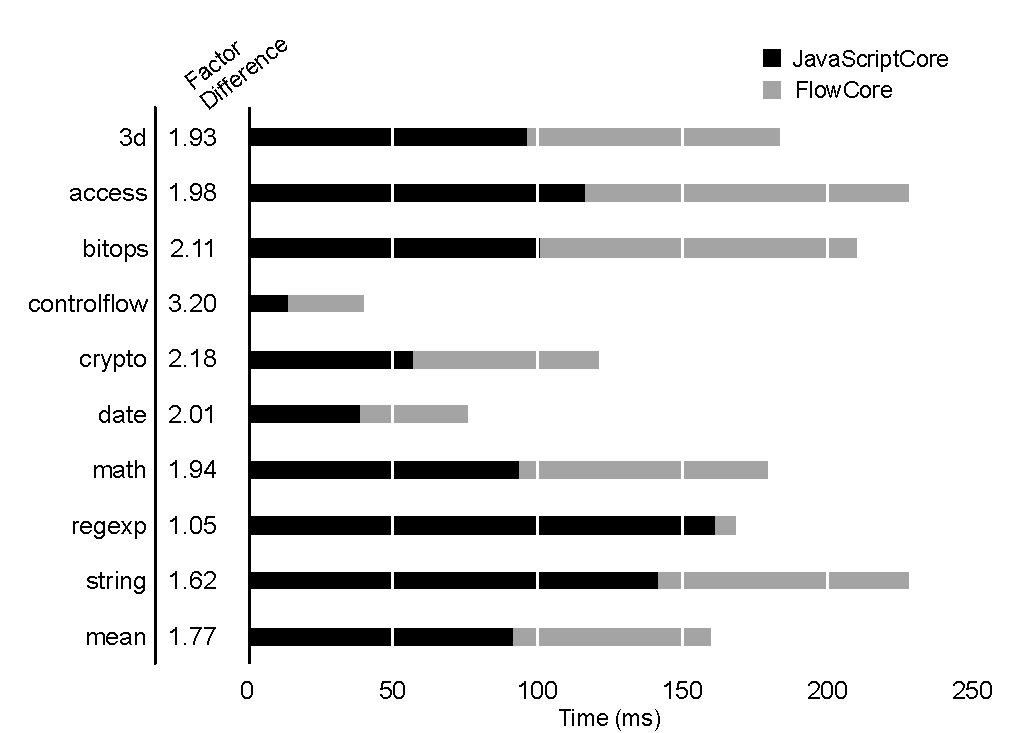
\includegraphics[width=\textwidth,keepaspectratio=true]{graphics/sunspider-jsc-vs-flowcore.pdf}
  \caption{SunSpider Benchmark results (interpreters only): JavaScriptCore vs. \JitFlow.}
  \label{fig:first-class-sunspider}
\end{figure}

\autoref{fig:first-class-sunspider} reveals overall execution speed of JavaScript benchmark results: \JitFlow\ has a mean execution time of 158.33~ms, whereas JavaScriptCore has a mean execution time 89.44~ms.
The SunSpider benchmark does not contain first-class labeling operations, so the overall 77\% slowdown represents the overhead incurred by \JitFlow's implementation of label propagation.
In comparison, other information flow approaches~\cite{just.etal+11} introduce a 150\% slowdown making programs two to three times slower.

%\JitFlow\ extends all values within the VM by 64 bits so that both JavaScript primitives and object references carry a label.
The bit vector representation permits \JitFlow\ to carry out label propagation via bitwise-or.
By packing the label into the \jsvalue (\autoref{sec:jitflow-labelencoding}), \JitFlow\ ensures that a full first-class label object exists only when explicitly constructed (\code{new} \FlowLabel) or retrieved (\mlabelof) by the developer.
As a result, the introduction of the first-class labeling system into the hosted environment incurs no additional runtime performance overhead compared to a fully automatic labeling system.
We do not evaluate the performance impact of evaluating functions attached to the network hook, because it remains insignificant within a debugging environment and the developer has the power to implement any monitor function they desire.
However, evaluating the monitor function will add overhead to all network requests.

The performance of the underlying labeling framework implies that even sites with large amounts of JavaScript code execute without noticeable slowdown.
To test whether the information flow tracking framework causes a noticeable performance decrease, we used \JitFlow\ to visit (and log into) JavaScript intensive sites, such as Facebook, GMail, Google Maps, Bing, GitHub and Cloud9 IDE.
These sites do not make use of the first-class labeling system introduced in this paper.
However, user interaction proves that the performance overhead of the labeling framework does not introduce any usability issues.

\subsection{Completeness}

To verify that the underlying framework does not introduce any runtime bugs when interpreting either machine-generated or human-written JavaScript found in the wild, we scripted the web browser hosting \JitFlow\ to automate the visiting of all sites in the Alex Top 500~\cite{alexa}.
This webcrawler injects code into each page, to perform two actions: (1) attach a network monitor and (2) fill out and submit the first form on the page using data labeled with an identifying principal.
The injected monitor verifies that the submitted form generates a request containing the identifying principal.
The automated crawl checks that \JitFlow's label propagation engine can execute JavaScript code in the wild.

The first-class labeling system also aided development of \JitFlow\ itself.
For each of the data-flow and control-flow features covered by the tracking engine (\autoref{ch:label-tracking}), we created a unittest case that ensures the semantic correctness of the applied labels.
The ability to apply labels to specific values, pass them through computation, and then verify that the attached labels upgrade accordingly proved exceedingly useful throughout the \JitFlow's development cycle.
Without first-class labels to assist in writing a unittest suite, we would feel far less confident of the \JitFlow's labeling capabilities.

\subsection{Security}

The labeling framework \JitFlow, generates, at runtime, new security principals for every unique label generated by the developer and new domain encountered by the web browser.
Introduction of runtime principals requires mutation of the \FlowLabelRegistry.
By design, \JitFlow\ does not support declassification, preventing a communication channel via the labeling framework itself.

\JitFlow's first-class labeling system exposes, to the web application and any injected code, a JavaScript API for creating and applying labels to JavaScript values.
This exposure represents a new attack surface that might allow an attacker to target the labeling framework itself.
However, we envision web developers using the first-class labeling system only in a testing environment, where it provides no benefit to the attacker.
Nevertheless, even when used by all clients, the lack of declassification means that the attacker-injected code cannot drop labels applied by the developer for debugging purposes.

Finally, the browser component allows registration of many monitor functions, through a JavaScript interface accessible by code injected into the web application.
It evaluates all monitor functions registered, in registration order.
The developer-supplied monitor function executes for as long as all previous monitors in the chain return \code{true}, indicating an allowable flow.
So, in the worst case, an attacker can register their own monitor function first, preempting the execution of the developer's monitor.
But this injection only allows the attacker to halt the chain by returning \code{false}, indicating a policy-violating flow.
Semantically, the system only considers an information flow allowable when \emph{all} monitors in the chain indicate success by returning \code{true}.

\subsection{Utility as a Debugging Tool}

To evaluate the first-class labeling system as a tool for testing web applications and discovering security vulnerabilities, we create a web page that contains a user login form.
Acting as a malicious developer, we insert code into the page, which uses the \code{sniffPassword} label dropping code (\autoref{list:sniffPassword}) prior to exfiltrating the form contents to a second server via both an \code{XmlHttpRequest} and as part of an \code{img.src} URL.
Acting as a security researcher, we mirror the page and add labeling code that applies a tag to the form's DOM node and a network monitor function that checks for the unique tag.
Visiting the mirrored page successfully triggers the monitor function, alerting us to the exfiltration.
WebKit's developer tools assisted with finding the portion of the page responsible for generating the image request.

For a more realistic example, we attempt a similar attack using a mirrored \url{ebay.com} page obtained from XSSed~\cite{xssed}, this time targeting the site's cookie.
This page loads content from several different sources, and contains an XSS vulnerability that we exploit to inject the exfiltration code.
Because the browser hosting \JitFlow\ automatically labels the cookie with the domain of origin, we did not need to insert labeling code.
Instead, we find it sufficient to implement a network monitor that checks only whether data sent to an origin does not contain third-party principals.
This monitor detected the exfiltration of the cookie (labeled with \url{ebay.com}) being sent to a server other than \url{ebay.com}.
Again, WebKit's developer tools assisted with pinpointing the JavaScript code responsible for the request.

%========================================================================

\section{Summary}
\label{sec:first-class-summar}

\JitFlow\ presents to the JavaScript developer a first-class labeling system that exposes an underlying information flow framework.
Developers can use their domain knowledge to label JavaScript values within their application and construct network monitor policies that selectively ignore automatically applied labels.
The labeling system provides dynamic creation of security principals, supporting the common practice of loading code and resources from many different domains in web applications.

\JitFlow\ introduces a new built-in \FlowLabelObject\ class to the hosted environment, which the developer uses to selectively label JavaScript values.
The developer creates \FlowLabelObject\ instances using existing JavaScript values as security principals or by composition with other \FlowLabelObject\ instances via the lattice \join\ method.
The \msubsumes\ method allows comparison of all \FlowLabelObject\ instances reporting their subset relation within the label lattice, while the strict equality operator (\code{===}) allows unique identification of labels by their internal bit vector representation.
Together with the ability to retrieve labels attached to values via the new built-in \mlabelof\ operator, \JitFlow\ gives the developer the means to implement security policies in JavaScript.

Because of the shared underlying data-structures, exposing the labeling framework as first-class language objects to the developer incurs no additional runtime cost compared to automatic labeling systems.
It allows developers to leverage their domain knowledge and existing JavaScript experience and direct their focus on identifying and debugging application specific information flows.
For sites that have large amounts of JavaScript code, the system can be used in a testing environment.
First-class labels allow developers to improve the security of their applications by writing policies in JavaScript that selectively ignore the high quantity of reports produced by automatically attached labels.

%========================================================================
\begin{comment}
\section{Tracking JavaScript Information Flows}

% Previous work~\cite{empirical-study} identifies history sniffing as the primary use of active implicit flows.

Label propagation within the JavaScript VM occurs at the construction of every temporary value.
As shown in \autoref{list:indirect-flows-functions}, it can track, at runtime, labels across multiple assignment statements and function calls.
The example shows that temporary computed values (those not assigned to a variable) also carry a label.
And that labels are propagated into, through, and from function calls.

\begin{lstlisting}[caption={Example Indirect Explicit Flows in Functions},label={list:indirect-flows-functions}]
> labelGood = new FlowLabel("good");

> function echoArgs(arg) {
>    print(labelof arg);
>    return arg;
> }
> echoArgs(labelGood(7));
  [FlowLabelObject good] // print arg
   7 [FlowLabel good]
  
> function applyLabel(arg) {
>    var labelBad = new FlowLabel("bad");
>    return labelBad(arg);
> }
> applyLabel(7)
  7 [FlowLabel bad]

> labelFoo = new FlowLabel("foo")
> labeledFunction = labelFoo(echoArgs);
> labeledFunction(7);
  [FlowLabelObject ] // print arg
  7 [FlowLabel foo]

\end{lstlisting}
\end{comment}

\begin{comment}
\subsection{Indirect Explicit Flows in Arrays}

We also handle some special fields, such as Array.length, and other operations, such as indexing (also on strings).

\begin{lstlisting}[caption{Example Indirect Explicit Flows in Array Objects},label={list:indirect-flows-arrays}]
> labelGood = new FlowLabel("good.com")
> myArray = labelGood([10,11,12,13,14]);

> myArray.length
  [TODO]

> myArray[3]
  13 [FlowLabel good]

> myArray[100]
  undefined [FlowLabel good]
\end{lstlisting}
\end{comment}

\begin{comment}
\subsection{Active Implicit Flows}

An example of such an implicit flow can be seen in the password sniffing code in \autoref{list:implicit-flow}.
Both the stopping condition of the loop, and the argument to the switch statement label the program counter with \textsf{good.com}.
Inside the switch, all assignments also carry the program counter label.

\begin{lstlisting}[caption={Example Indirect Explicit Flow},label={list:implicit-flow}]
> labelGood = new FlowLabel("good.com")
> password = labelGood("o24sk09nk12")

> function sniffPassword(pw) {
>     spw = "";
>     for (var i = 0; i < pw.length; i++) {
>         switch(pw[i]) {
>         case 'a':
>            spw += 'a';
>         case 'b':
>            spw += 'b';
>         ... // other characters elided
>         }
>    }
>    return spw;
> }

> sniffPassword(password);
  42 [FlowLabel good.com]
\end{lstlisting}

\end{comment}

\begin{comment}
\subsection{Property Hijacking Attack}

\todo{this example doesn't really motivate first-class labels. How to change it? write checks around uses?}
As documented by Chess et al.~\cite{js-hijacking} it is possible for attackers to hijack the getter and setter functions on native object prototypes such as \textsf{Object} and \textsf{Array}.
For example, in \autoref{list:prototype-hijacking} the attacker modifies \textsf{Object.prototype} such that it will run the \textsf{stealPassword} function whenever any object's \textsf{password} field is updated.
A real attack would have \textsf{stealPassword} communicate its argument back to an attacker controlled server, via a network request.
Because attacker supplied code is used to perform the hijacking, our labeling system causes the \textsf{\_\_password} field to carry the attacker's label.

\begin{lstlisting}[caption={Example Prototype Hijacking Attack},label={list:prototype-hijacking}]
Object.prototype.__defineSetter__("password",
  function(x) {
    stealPassword(x);
    this.__password = x;
  })

Object.prototype.__defineGetter__("password",
  function() {
    return this.__password;
  })
\end{lstlisting}


\begin{figure*}[ht]
  \centerline{\includegraphics[width=18cm,keepaspectratio=true]{graphics/example.pdf}}
  \caption{write text here.}
  \label{fig:example}
\end{figure*}

\end{comment}

\begin{comment}
\subsection{Monitoring the Flow}

\todo{how often is it the case that a secret was involved in early control flow. example: password-based login determines whether app gets run. A successful login taints app execution.}

** Example
  1. taint a pin, and have network traffic: can detect when it gets passed through the network
     (no) at each ajax request, developer can add a if-else label detection check
     (yes) at each request, browser uses config file to check them all (ship policy in the head, ref related work)
  2. malicious script tries to grab value directly
  3. malicious script tries to grab value through indirect flow

  - developer knows their framework, and can label the form fields where user enters sensitive data
  - can also happen via js plugins (greasemonkey) 

  : shim form entry, catch that users don't input pin in email or other field, via regex/js labeler
\end{comment}

\begin{comment}
*** Weaknesses
  - developer might forget to label a sensitive value
  - developer has to put in the checks, what if they forget one? [browser shim network]
    - if they have to put in the checks, what if attacker includes an ajax request? does it get around the checks?
  - site could shim the request object, but they'd have to get there first (before attacker);
  - could check all network traffic, and report all labels (developer can filter out what they want)

  - might be lots of work for developer
    : but can have default whitelist/self-domain policy, the network monitor optional
\end{comment}

\begin{comment}
\subsection{Security Analysis}

%*** Demonstrate tagging and inspecting values
%    Example of something first class labels can do that couldn't be done before
%    : done in example
%*** Performance (Sunspider, v8, craken, and (not honest) Dromaeo)
%    - need complete vs selective labeling
%*** What can first class labels do that other Systems can't?
%    - programmer can specify which values to track
%    nice to get list of all affected variables?
%*** Demonstrate lower false positive rate
%    - shim the network traffic to label some objects on large site (facebook)
%*** Measure the number of useful vs nop label operations
%    => quantifies argument for sparse labeling
%       and vm-level optimizations
%*** Prevent leak of tainted data in a custom mashup!
%
%3 dimensions (plot triangle)
%- perf
%- security
%- developer effort 

\end{comment}

